\documentclass[border=3pt]{standalone}
\usepackage{amsmath,amssymb}
\usepackage{tikz}
\usetikzlibrary{arrows.meta}
\definecolor{cfg}{HTML}{2F7D4F}\definecolor{mcfb}{HTML}{2166AC}\definecolor{negr}{HTML}{A5352C}
\definecolor{inkc}{HTML}{1B1B1B}\definecolor{greyc}{HTML}{6F6F6F}
\begin{document}
\hyphenpenalty=10000\exhyphenpenalty=10000
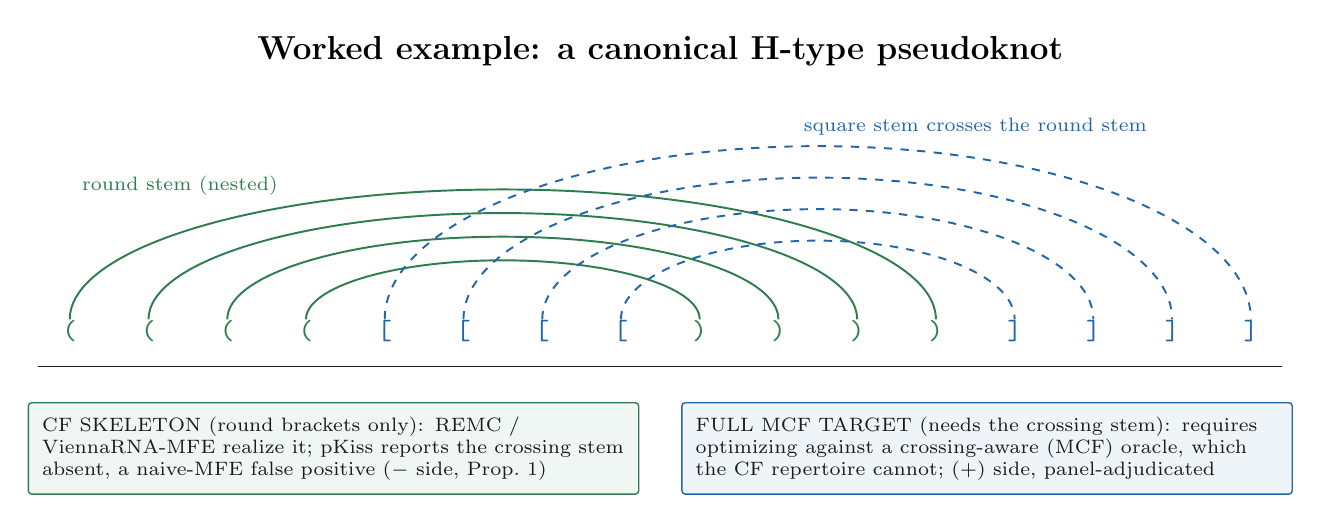
\begin{tikzpicture}[font=\footnotesize,
  b/.style={draw, rounded corners=1.2pt, align=left, inner sep=5pt, line width=0.5pt, text=inkc, font=\scriptsize}]
\node[font=\large\bfseries] at (8.5,3.55) {Worked example: a canonical H-type pseudoknot};
% dot-bracket glyphs
\foreach \k in {1,2,3,4} \node[cfg, font=\ttfamily] at (\k,0) {(};
\foreach \k in {5,6,7,8} \node[mcfb, font=\ttfamily] at (\k,0) {[};
\foreach \k in {9,10,11,12} \node[cfg, font=\ttfamily] at (\k,0) {)};
\foreach \k in {13,14,15,16} \node[mcfb, font=\ttfamily] at (\k,0) {]};
\draw[inkc, line width=0.5pt] (0.6,-0.45)--(16.4,-0.45);
% round (nested) arcs
\foreach \i/\j in {1/12,2/11,3/10,4/9}
  \draw[cfg, line width=0.7pt] (\i,0.15) arc(180:0:{(\j-\i)/2} and {(\j-\i)*0.15});
% square (crossing) arcs, dashed
\foreach \i/\j in {5/16,6/15,7/14,8/13}
  \draw[mcfb, line width=0.7pt, dashed] (\i,0.15) arc(180:0:{(\j-\i)/2} and {(\j-\i)*0.20});
\node[cfg, font=\scriptsize] at (2.4,1.85) {round stem (nested)};
\node[mcfb, font=\scriptsize] at (12.5,2.6) {square stem crosses the round stem};
% verdict boxes
\node[b, draw=cfg, fill=cfg!7, text width=74mm, anchor=north] at (4.35,-0.9)
  {CF SKELETON (round brackets only): REMC / ViennaRNA-MFE realize it; pKiss reports the crossing stem absent, a naive-MFE false positive ($-$ side, Prop.~1)};
\node[b, draw=mcfb, fill=mcfb!7, text width=74mm, anchor=north] at (12.65,-0.9)
  {FULL MCF TARGET (needs the crossing stem): requires optimizing against a crossing-aware (MCF) oracle, which the CF repertoire cannot; (+) side, panel-adjudicated};
\end{tikzpicture}
\end{document}
